%\VignetteIndexEntry{Glimma Vignette}
%\VignetteKeyword{RNA-Seq}
%\VignetteKeyword{differential expression}
%\VignetteKeyword{interactive graphics}
%\VignettePackage{Glimma}
%\usepackage[utf8]{inputenc}
\documentclass{article}

\RequirePackage{/usr/local/lib/R/site-library/BiocStyle/resources/tex/Bioconductor}

\AtBeginDocument{\bibliographystyle{/usr/local/lib/R/site-library/BiocStyle/resources/tex/unsrturl}}
\usepackage{hyperref}
\usepackage{graphicx}
\newcommand{\Rarg}[1]{\textcolor{BlueGreen}{{\sf{#1}}}}
\newcommand{\Rfun}[1]{\textcolor{VioletRed}{{\sf{#1}}}}

\usepackage{Sweave}
\begin{document}
\input{Glimma-concordance}

\title{Glimma: interactive graphics for differential expression analyses of RNA-seq data}
\author{Shian Su, Charity W. Law, Matthew E. Ritchie}
\date{First edition 28 January, 2016\\
Last revised \today}
\maketitle

\tableofcontents

\section{Quick start}\label{sec:quickstart}
\Biocpkg{Glimma} is a \Bioconductor{} package for interactive visualization of results from differential expression analyses of RNA-sequencing (RNA-seq) data. Its functionality is intended to enhance reporting capabilities so that such results can be explored more conveniently by end-users. Glimma, which loosely stands for interactive {\bf G}raphics from {\bf limma}, extends some of the popular plotting capabilities in the \Biocpkg{limma} \cite{limma} package such as multi-dimensional scaling (MDS) plots and mean-difference (MD) plots. Glimma is designed to handle objects native to limma, as well as from \Biocpkg{edgeR} \cite{edgeR} and \Biocpkg{DESeq2} \cite{DESeq2} packages, with its output as a html page containing interactive displays (Figure~\ref{fig:overview}).
Displays within Glimma were inspired by visualisations from {\it Degust} software \cite{Degust}.

\begin{figure}[!ht]
  \centerline{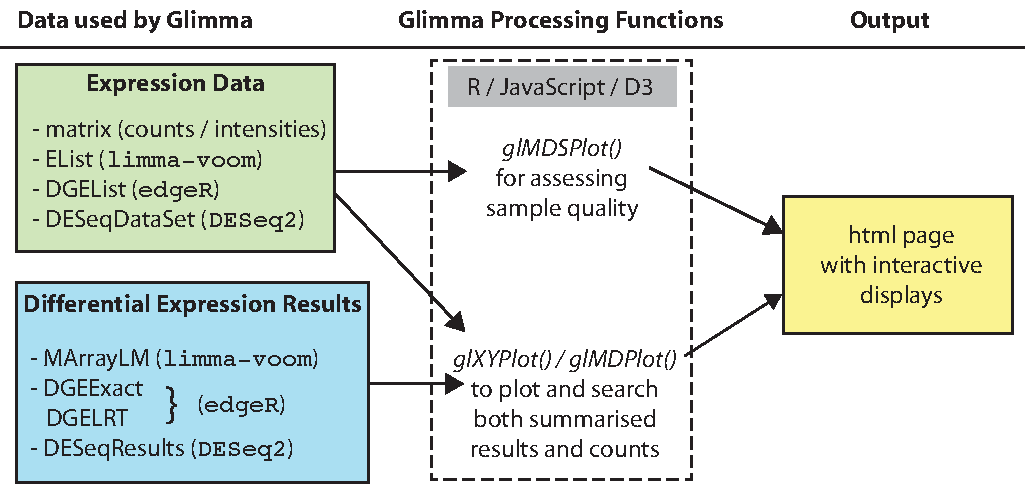
\includegraphics[width=0.65\linewidth]{GlimmaWorkFlow.pdf}}
  \caption{Overview of workflow showing the input and output types for Glimma.}
  \label{fig:overview}
\end{figure}

The main dataset used in this vignette is taken from an RNA-seq experiment examining lymphoma cell-lines in mice with alterations to the Smchd1 gene \cite{Smchd1}. The data is available for 4 wildtype samples and 3 samples with null levels of Smchd1. The count data is available within Glimma and is stored as a {\sf DGEList} object that is native to edgeR. In our analysis, we begin by removing lowly expressed genes and by performing TMM-normalisation \cite{tmm}.

\begin{Schunk}
\begin{Sinput}
> set.seed(20161000)
> options(digits=2)
> library(Glimma)
> library(limma)
> library(edgeR)
> data(lymphomaRNAseq)
> rnaseq <- lymphomaRNAseq
> rnaseq <- rnaseq[rowSums(cpm(rnaseq)>1)>=3,]
> rnaseq <- calcNormFactors(rnaseq)
\end{Sinput}
\end{Schunk}

\begin{figure}[!ht]
  \centerline{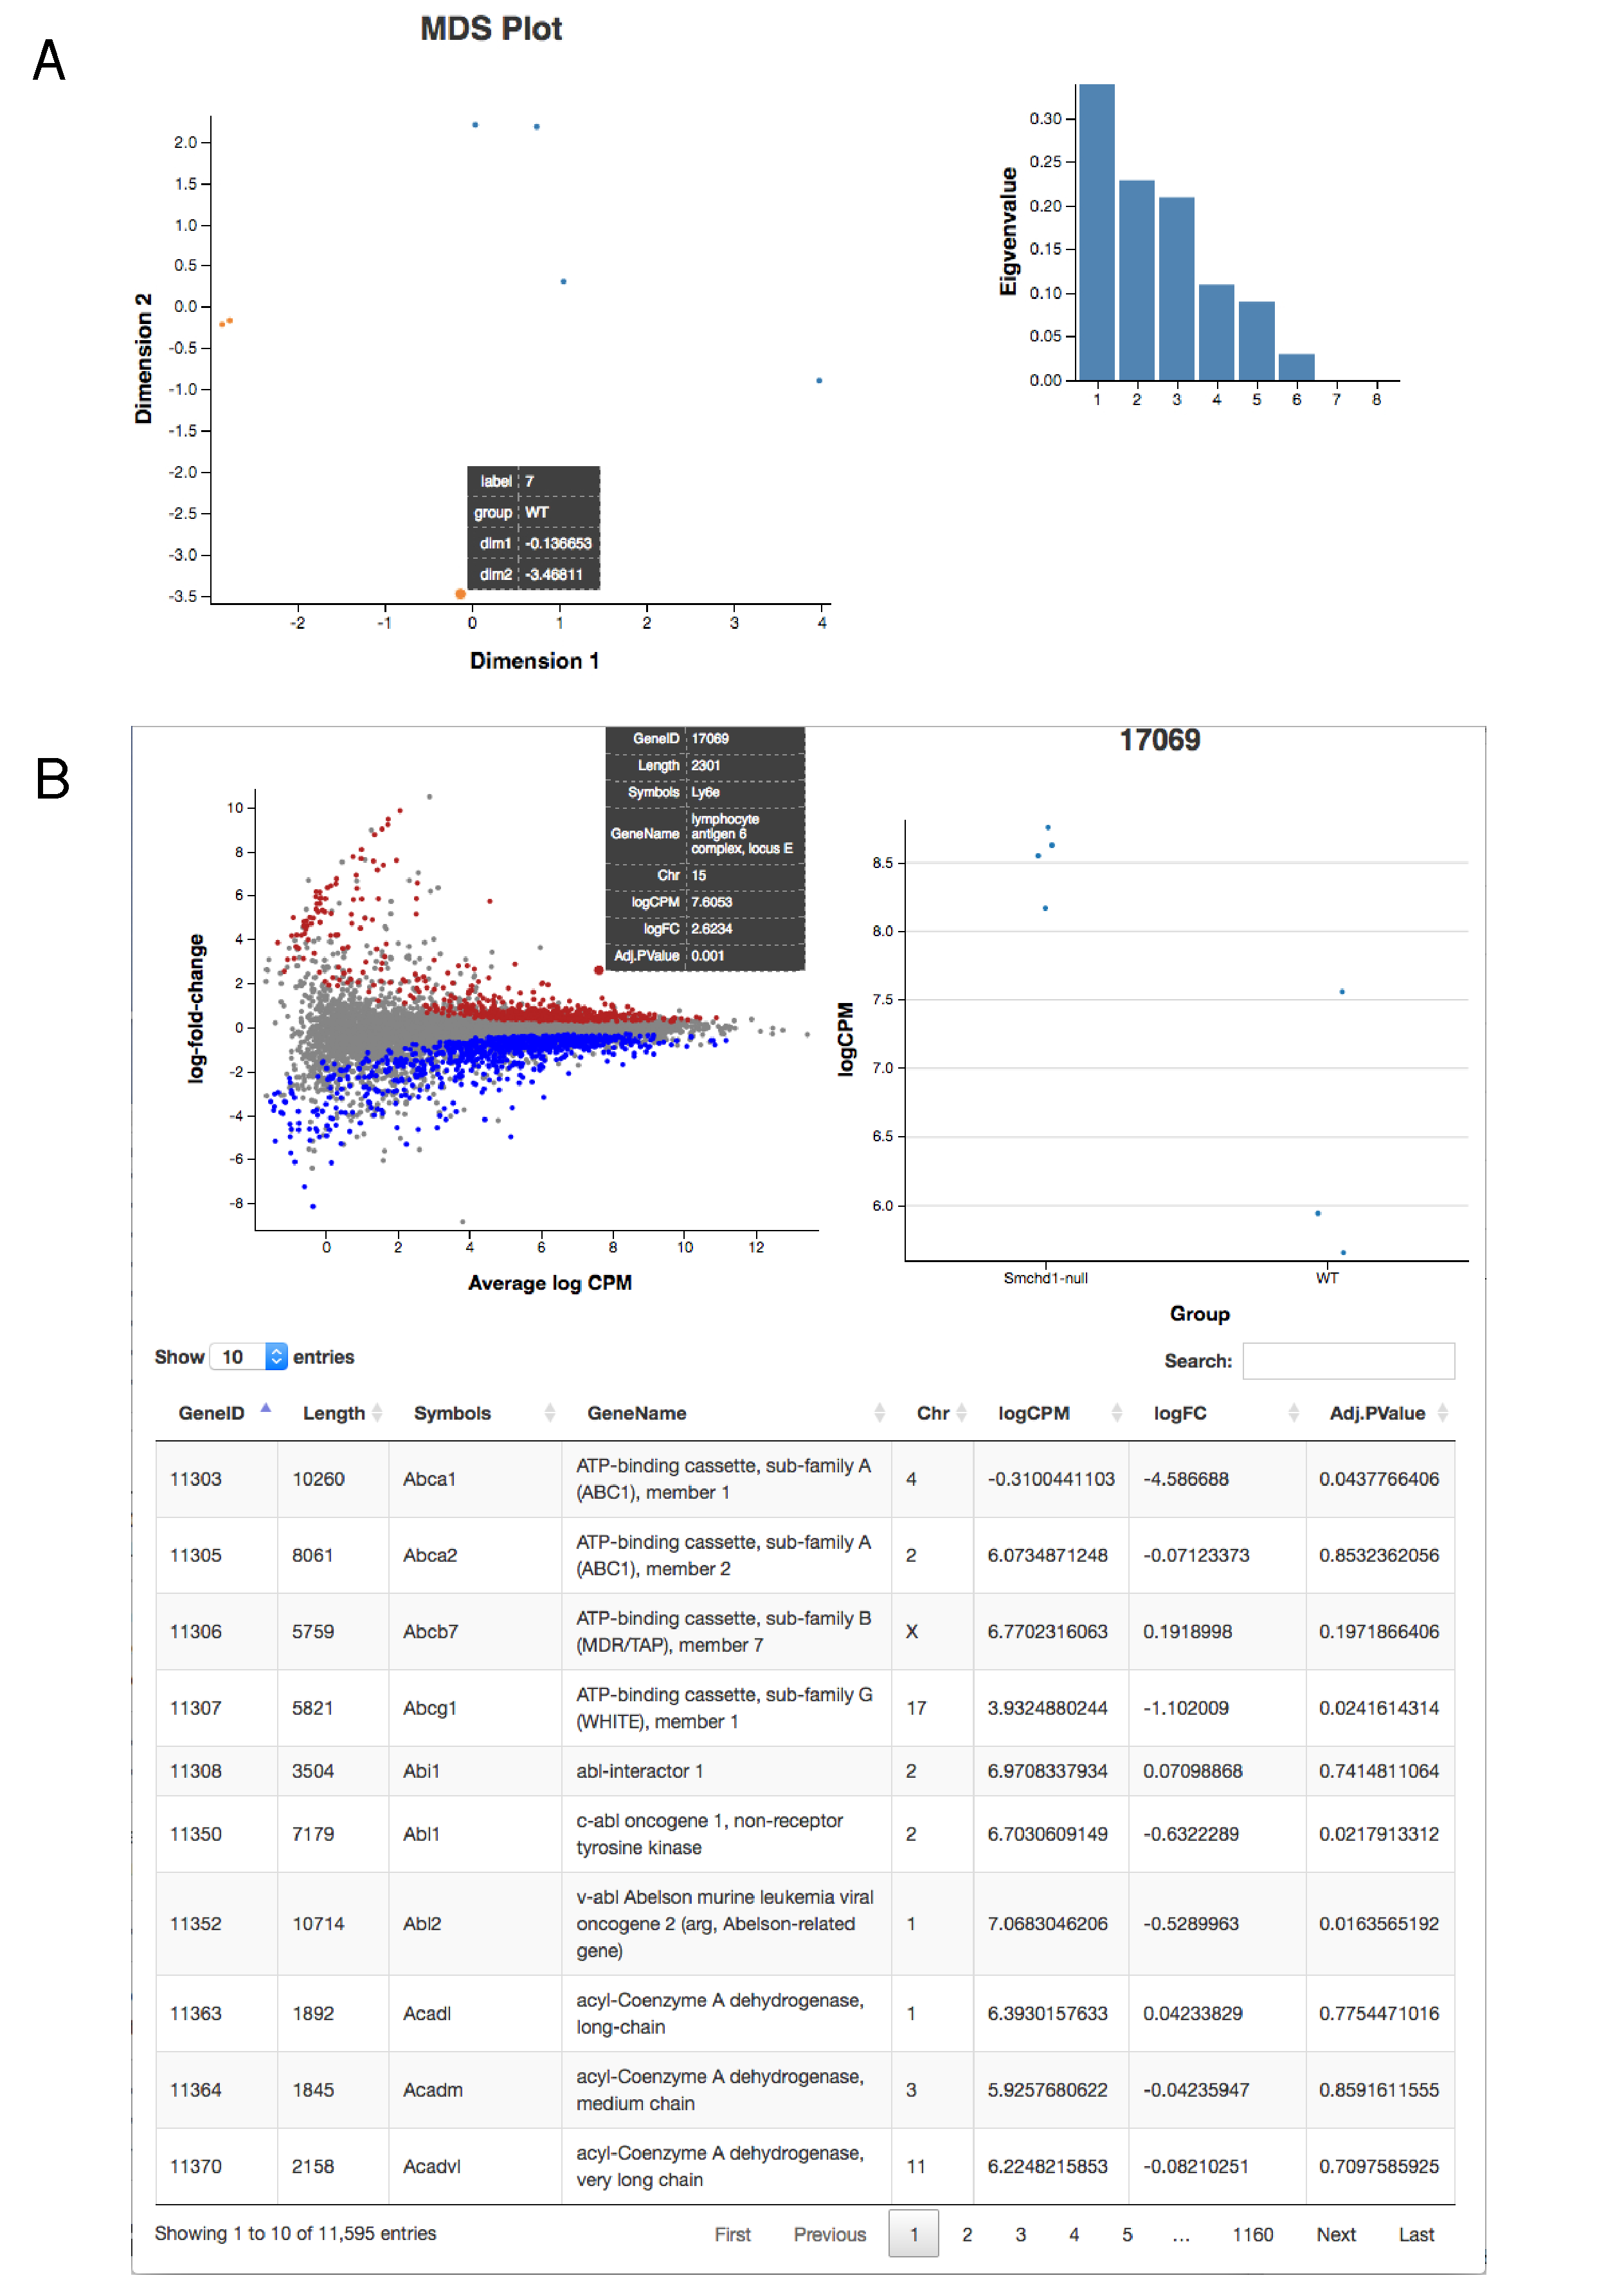
\includegraphics[width=0.7\linewidth]{quickstart.pdf}}
  \caption{A. Interactive MDS plot where the dimensions displayed in the MDS plot (left) can be changed by clicking on the associated bars in the barplot (right). B. Interactive MD plot where gene-wise logFCs are plotted against mean expression values (top left). The expression of individual samples are displayed (top right) by selecting an associated gene within the MD plot. A table of gene-wise information is displayed in the table (bottom), where genes and keywords can be searched specifically using the Search-bar.}
  \label{fig:quickstart}
\end{figure}

Using the \Rfun{glMDSPlot} functon, an interactive MDS plot can be created to examine the clustering of samples in an unsupervised fashion. Distances in the plot are used to represent similarities and dissimilarities between samples. Glimma's MDS plot allows users to interactively browse through different dimensions of the plot (Figure~\ref{fig:quickstart}A). Note that {\sf {\bf rnaseq}} is an {\sf DGEList} object.
\begin{Schunk}
\begin{Sinput}
> groups <- rnaseq$samples$group
> groups
\end{Sinput}
\begin{Soutput}
[1] Smchd1-null Smchd1-null Smchd1-null Smchd1-null WT          WT          WT         
Levels: WT Smchd1-null
\end{Soutput}
\begin{Sinput}
> glMDSPlot(rnaseq, groups=groups)
\end{Sinput}
\end{Schunk}

A limma-style analysis is carried out using voom with quality weights \cite{voom, voomqwts}, testing for the differential expression of genes between Smchd1-null and wildtype samples. For simplicity the rest of this article mostly uses limma objects to demonstrate the usage of Glimma, but Glimma works just as well on output from edgeR and DESeq2, where examples are shown explicitly in Sections~\ref{sec:appendix}. Using an adjusted p-value cutoff of 5\%, 882 genes are detected as down-regulated in the Smchd1-null group relative to wildtypes, and 634 genes as up-regulated.
\begin{Schunk}
\begin{Sinput}
> design <- model.matrix(~groups)
> colnames(design) <- c("WT", "Smchd1null.vs.WT")
> vm <- voomWithQualityWeights(rnaseq, design=design)
> fit <- lmFit(vm, design=design)
> fit <- eBayes(fit)
> dt <- decideTests(fit)
> summary(dt)
\end{Sinput}
\begin{Soutput}
      WT Smchd1null.vs.WT
-1   128              882
0    629            10079
1  10838              634
\end{Soutput}
\end{Schunk}

The results of the analysis can be examined more thoroughly through the use of Glimma's interactive MD plot which shows gene-wise log$_2$-fold changes (logFCs) plotted against average expression values and associate these to sample-specific expression values. This allows users to see summarised results from all the genes as a whole whilst being able to scrutinise the expression of individual genes at the same time. To do this, Glimma's \Rfun{glMDPlot} function is used, where significantly up- and down-regulated genes can be highlighted in red and blue respectively (Figure~\ref{fig:quickstart}B). Note that {\sf {\bf fit}} is an {\sf MArrayLM} object and {\sf {\bf dt}} is a {\sf TestResults} object.
\begin{Schunk}
\begin{Sinput}
> glMDPlot(fit, status=dt, counts=rnaseq$counts, groups=groups)